\input{mmd-memoir-header}
\def\bibliostyle{plain}
\def\bibliocommand{\bibliography{library.bib}}
\def\mytitle{3 Month Report}
\def\myauthor{M.A.Rol}
\def\latexmode{memoir}
\input{mmd-memoir-begin-doc}

\title{\huge{Quantum Error Correction with Spins in Diamond}  \\  \large{3 month report}}
\author{Adriaan Rol \\  Team Diamond, Delft University of Technology}
\date{\today}
\maketitle 
\newpage
\tableofcontents
\mainmatter


\chapter{Introduction}
\label{introduction}

The question whether an arbitrary quantum state can be protected against its environment is not only fundamentally interesting but also of practical significance when considering the feasibility of a quantum computer. Correcting quantum errors is a stepping stone on the way to fault tolerant quantum computation~\citep{Nielsen2010}. 

An interesting candidate for quantum error correction is the negatively charged Nitrogen Vacancy (NV-) centre in diamond. The NV- centre is a naturally occurring impurity in diamond that we can address and control~\citep{Childress2013}. It behaves much like a single ion or small molecule that sits in a protective environment of mostly spin-less carbon--12 atoms that it does not strongly interact with~\citep{Bernien2014}. The fact that we can control carbon--13 atoms in its environment~\citep{Taminiau2012} gives us the necessary extra qubits to attempt quantum error correction. 

Combined with the linking of such systems~\citep{Bernien2013} the NV- centre is a promising candidate for a topological quantum computer as proposed by Nickerson et al.~\citep{Nickerson2013}. 

Experiments demonstrating a form of quantum error correction have been demonstrated in a variety of systems. Codes correcting for one type of error have been implemented with nuclear magnetic resonance~\citep{Cory1998}~\citep{Moussa2011}, trapped ions~\citep{Schindler2011} and superconducting circuits~\citep{Reed2012}. Recently two groups have implemented a gate based quantum error correction scheme with NV- centres~\citep{Taminiau2014}~\citep{Waldherr2014}. We will build upon this work and attempt a measurement based algorithm. 

\chapter{Quantum Error Correction using Spins in Diamond}
\label{quantumerrorcorrectionusingspinsindiamond}

\section{Quantum Error Correction}
\label{quantumerrorcorrection}

\subsection{Classical Majority Voting}
\label{classicalmajorityvoting}

In order to understand Quantum Error Correction (QEC) it is useful to first understand classical error correction. A classical bit can be either a 1 or a 0. If an error occurs a 1 turn into a 0 and vice versa. This type of error is known as a bit flip. 

One of the crudest ways to correct for classical errors is majority voting. The logical bit is encoded onto multiple bits and sent. Upon arrival the original logical bit is recovered by measuring all bits and going with the majority. 

\subsection{The Concept of Quantum Error Correction}
\label{theconceptofquantumerrorcorrection}

The principle of QEC is very similar but has two extra difficulties. One cannot measure the state of a qubit without disrupting it and instead of one type of error that is discrete, there are three types of errors that grow continuously. The three types of error are the bit-flip, the phase-flip and the combination of the two. 

The key to QEC is the way the errors are diagnosed. Instead of measuring each qubit separately, parity measurements are performed on pairs of qubits. Not only is no information about the state of the qubits extracted, but the measurement also projects the qubits onto the error basis, making the errors discrete. By comparing parity measurements we can determine if an error has occurred and correct for it. 

Three qubits are required to correct for one type of error. By encoding onto five or more qubits and performing parity measurements in different bases one can correct for arbitrary errors. 

\subsection{Quantum Error Correction Schemes}
\label{quantumerrorcorrectionschemes}

The simplest example of a quantum error correction code is the three qubit gate-based circuit as seen in (\autoref{fig:3qb_gb_qec}). It consists of the same basic steps as the classical error correcting scheme. First the state of the qubit  $\alpha | 0 \rangle+ \beta |1\rangle $ is encoded onto the entangled logical qubit state $ \alpha |000\rangle + \beta | 111 \rangle $. After that the qubit is `protected' by the redundancy of the logical qubit. 

In the last stage the logical qubit is first decoded and then corrected. If a bit flip has occurred on one of the qubits the last Toffoli gate will correct the decoded qubit. By inserting Hadamard gates immediately after encoding and just before decoding this scheme can be used to correct for phase-flips instead of bit-flips. 

This gate based quantum error correction circuit has two drawbacks. If one wants to correct for an error the logical qubit has to be decoded, losing the desired protection against errors. Secondly the errors accumulate in the outer qubits making it hard to repeat this scheme as these qubits need to be reinitialised every time the scheme is run.

\begin{figure}
        \centering
        \subbottom[Three qubit gate based quantum error correction \label{fig:3qb_gb_qec}]
                {\includegraphics[width=0.3 \textwidth]{3qubitGateBasedQEC.png}}
        \subbottom[Three qubit measurement based quantum error correction \label{fig:3qubitmb_qec}]   {\includegraphics[width=0.5 \textwidth]{3qubitMB_QEC.png}}
 \caption{Three qubit error correction codes, a comparison of the gate based and measurement based code. }\label{fig:qec_circuit}
\end{figure}


These issues are addressed in a scheme that employs measurements on ancilla qubits (\autoref{fig:3qubitmb_qec}). By performing a parity measurement on an ancilla qubit and correcting depending on its outcome the logical qubit does not have to be decoded in order to protect against errors, thus remaining in its protected state. Because the ancillae are measured they are easy to reset allowing the error correction scheme to be repeated. 

The measurement based scheme forms the basis of more complex error correcting codes that can correct for arbitrary errors. These schemes are based on the same principles as the 3 qubit code but rely on more complex logical qubit states and operations on the ancillae to correct for errors. 

When qubit operations are performed on the logical qubits, the need for decoding to apply operations disappears. Combined with a scheme where the error correction can be repeated this brings fault-tolerant quantum computation a step closer~\citep{Nielsen2010}. The 7-qubit code devised by Andrew Steane is the current favourite for quantum error correction because it enables basic operations on the logical qubit in a straightforward way~\citep{Mermin2007}. 

\section{Controling Spins in Diamond}
\label{controlingspinsindiamond}

The Nitrogen Vacancy centre in diamond is a well investigated system~\citep{Doherty2013a} and a promising candidate for quantum computation~\citep{Childress2013}. In order to implement three qubit measurement based QEC we need three qubits plus ancillae that we can initialise, measure and conditionally perform operations on. These extra qubits are found in Carbon--13 atoms, which are normally a source of decoherence. These atoms can be addressed using a resonant decoupling sequence~\citep{Taminiau2012}. 

It has been shown that the nuclear- and electron- spin-state of the NV- centre can be initialized, coherently controlled and read-out using microwaves and laser pulses~\citep{Robledo2011}. These are essential tools in controlling the NV- centre. In this chapter I will explain how control over the electron-spin-state can be used to address weakly coupled Carbon--13 atoms. 

\subsection{Spin Control}
\label{spincontrol}

The electronic ground state Hamiltonian can be written as~\citep{Pfaff2013}:
 \begin{equation} 
H_{GS} = \Delta {S_z}^2 + \gamma_e \mathbf{B} \cdot \mathbf{S}
\end{equation}

With zero field splitting $\Delta \approx 2.88 \mathrm{GHz}$  and gyromagnetic ratio $\gamma_e  = 2.802$ MHz/G . In this expression the interactions with the Nitrogen nucleus and the Carbon spin bath are not included. By applying a magnetic field $B_z$ a long the N-V axis the degeneracy of the  $m_s =\pm1$ states is lifted by the Zeeman effect. A two level system that serves as a qubit can be defined with  $m_s=0:=|0\rangle$ and $m_s = -1 := |1\rangle$. 

On the bloch-sphere the state vector rotates around the quantisation axis with a frequency depending on the energy splitting of the two states given by the Larmor frequency  $\omega_L =\Delta - \gamma_e {B_z} $.\footnote{When  $\omega_L$  is used as a vector it is pointing in the $\hat{z}$ direction.} By applying an external field a term is effectively added to the Hamiltonian, changing the quantisation axis and thereby its evolution. By applying microwaves with the right frequency this can be used to selectively drive the transition from the  $|0\rangle$ state to the $|1\rangle$state~\citep{Jelezko2004}. 

In a similar fashion the state of a Carbon--13 atom can be controlled by switching an additional term in the Hamiltonian on and off. The Hamiltonian of the nuclear spin depends on the electron state~\citep{Taminiau2012}:
 \begin{eqnarray}
H_0= \gamma_C B_z I_z \\
H_1 = \gamma_C B_z I_z +H_{HF} = \gamma_C B_z I_z+ A_\parallel I_z + A_\perp I_x
\end{eqnarray}

The the hyperfine term is not present when the electron is in the $m_s = 0$ state. The hyperfine term consists of a contact term and a dipole term. For carbons with weak couplings (A$<$200kHz) the contact term is expected to be negligible and the dipole term is given by~\citep{DeLange2012}:

\begin{equation}
H_{dip} = \frac{\mu_0 \gamma_e \gamma_C \hbar^2 }{4 \pi r^3} [ \mathbf{S \cdot I} - 3 (\mathbf S \cdot \hat{n_{hf}})(\mathbf I \cdot \hat{n_{hf}})] 
\end{equation}

From this equation the parallel and orthogonal components of the Hyperfine interaction, with respect to the N-V axis along the z direction, can be derived to be:
 \begin{eqnarray}
A_\parallel= - \frac{\mu_0 \gamma_e \gamma_C \hbar^2 }{4 \pi r^3} \left(3\cdot \frac{z^2}{r^2}-1\right)\\
 A_\perp =  -\frac{\mu_0 \gamma_e \gamma_C \hbar^2 }{4 \pi r^3}\left( 3\cdot\frac{\sqrt{x^2+y^2}\cdot z}{r^2}\right)
\end{eqnarray}


\begin{figure}[htbp]
\centering
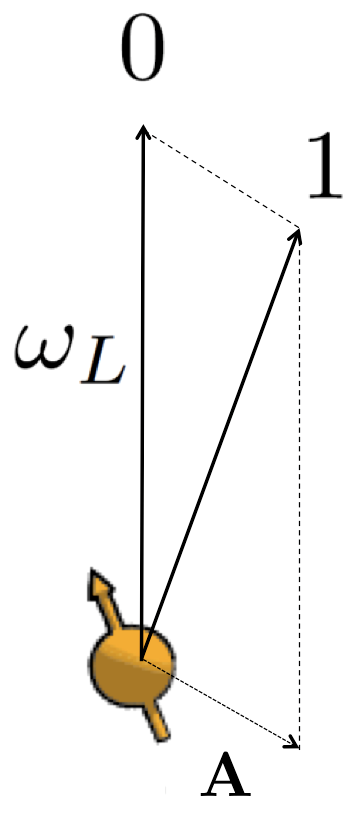
\includegraphics[keepaspectratio,width=0.2\textwidth,height=0.75\textheight]{QuantizationAxis.png}
\caption{Flipping the electron spin from the  $m_s=0$ to the $m_s= -1$ state changes the quantization axis of $^{13}\mathrm{C}$ nuclear spins. For  $m_s=0$ spins precess about $\omega_L$. For  $m_s=-1$ spins precess about a distinct axis $\mathbf{\tilde{\omega}}=\mathbf{\omega_L} +\mathbf{A}$~\citep{Taminiau2012} }
\label{fig:quantax}
\end{figure}



\subsection{Controlling a Carbon through Dynamical Decoupling}
\label{controllingacarbonthroughdynamicaldecoupling}

To understand how a Carbon--13 atom can be controlled it is useful to consider three situations. In the first situation $\omega_L$ and $\mathbf{A}$ point in the same direction. In the second situation $\omega_L$ and $\mathbf{A}$ are of comparable magnitude and point in different directions, resulting in a big angle between the quantisation axes. In the last situation $A$ is small compared to  $\omega_L$ resulting in a small angle between the quantisation axes.

When applying a decoupling sequence with N\slash 2 decoupling units of the form \mbox{$\tau - \pi -2\tau-\pi-\tau$} the nuclear spin alternately rotates around the  $\omega_L$ and the $\tilde{\omega}$ axis. The net result of one such decoupling sequence is a rotation around an axis  $\mathbf{\hat{n_i}}$ by an angle $\phi$  . Where  $\mathbf{\hat{n_i}}$  depends on the initial state of the electron~\citep{Taminiau2012}. 

When $\mathbf{\omega_L}$ and $\mathbf{A}$ point in the same direction, the net rotation axes are parallel making it impossible to control the Carbon--13 atom using this decoupling sequence. 

In the case where $\omega_L$ and $\mathbf{A}$ are of comparable magnitude the net rotation axes  $\mathbf{\hat{n_i}}$ are strongly dependent on the initial state for almost any inter-pulse delay $\tau$. Although this sounds nice as entanglement is almost always created, having two or more carbons with couplings comparable to the Larmor frequency creates complicated interactions. 

When considering the case where $\mathbf{A}$ is small compared to  $\omega_L$ the net rotation axes  $\hat{n_0}$ and $\hat{n_1}$ are practically parallel and the nuclear spin undergoes an unconditional evolution. Only when the inter-pulse delay is precisely resonant with the spin dynamics the axes are antiparallel leading to a conditional rotation. The resonant condition occurs at~\citep{Taminiau2012}: 

 \begin{equation}
\tau = \frac{(2k+1)\pi}{2 \gamma_C B_z + A_\parallel}
\label{eq:res_dip_loc}
\end{equation}

And for $\omega_L \gg \mathbf{A}$ the dip has a width of:

 \begin{equation}
\Delta = \frac{A_\perp}{2\cdot (\gamma_C B_z)^2}
\label{eq:res_dip_width}
\end{equation}

If  $\hat{n_0}$ and $\hat{n_1}$ are not parallel, the resulting conditional rotation of the nuclear spin generally entangles the electron and nuclear spins. As a result, for an unpolarised nuclear spin state, the final electron spin state is a statistical mixture of $|x\rangle$ and $|-x\rangle$ when starting from the $|x\rangle$  state. Where the probability that the initial state is preserved is given by: 


\begin{equation}
P_x = (M+1)/2 
\end{equation}

With for a single nuclear spin: 


\begin{equation}
M = 1-(1 - \hat{\mathbf{n_0}} \cdot \hat{\mathbf{n_1}}) \sin^2 \frac{N\phi}{2}
\end{equation}

\subsection{How many C13 can we control?}
\label{howmanyc13canwecontrol}

In reality the electron is not interacting with one carbon but with a bath of carbon atoms. When the electron interacts with multiple carbons at the same time M is given by the product of all individual values $M_j$ for each individual spin j. In order to coherently control one carbon the electron should not entangle with any other carbon when addressing it. 

In practice this means that the presence of a carbon that is strongly coupled (with respect to the Larmor frequency) makes it very hard to address any other carbon as entanglement is almost always created. It also means that resonances of weakly coupled (with respect to the Larmor frequency) carbons must not overlap. This excludes those carbons that are very weakly coupled in absolute terms as resonances of these carbons are located closely together.

As carbon--13 atoms are randomly distributed in the crystal the amount of weak resonances that can be addressed varies from NV to NV. By increasing the magnetic field the width and the delay-time of the resonances decreases. The downside is that it becomes harder to address these resonances as the resolution of the AWG used to apply the pulses is finite. 

The question wether we can address enough carbon atoms to perform 3-qubit measurement-based quantum error correction was investigated using simulations and will be discussed in the next chapter. 

\chapter{Simulating Carbon--13 Control}
\label{simulatingcarbon-13control}

Because the number of addressable carbon--13 atoms depends on their distribution within the crystal there is a high variability between NV- centres. Understanding a specific NV- centre tells you little about the ensemble of NV- centres. To address this issue Monte-Carlo type simulations where run so that statistics could be generated. 

The goal of these simulations is to a) get understanding of the physics involved in addressing carbon--13 atoms through dynamical decoupling sequences, b) determine if the project is feasible, and c) what the optimal experimental conditions would be to attempt 3-qubit measurement based quantum error correction. 

In this chapter I will first explain how the model works, what parameters where used and how sensitive the model is to the assumptions that where made. After that I will go into the results of the simulations, explain our hypotheses as to the physical processes leading to these results, and draw conclusions with respect to the optimal parameters. I will end with summarising how the model could be improved, and what the feasibility and priority of these improvements is. 

\section{Workings of the simulation}
\label{workingsofthesimulation}

In the simulations multiple NV- centres where generated with randomly distributed carbon--13 atoms within a radius dependent on the concentration. This radius was \ensuremath{\sim}6nm for the natural concentration ($\mu = 1.1\%$) of carbon--13. For each carbon the hyperfine interaction and the resonant decoupling conditions where calculated. The fidelity with which these carbons could be addressed was calculated by taking the interaction of the electron with the spin bath into account. Interactions between carbon atoms where ignored in this simulation. Based on these simulations statistics where gathered about the number of addressable carbon--13's. 

\begin{figure}[htbp]
\centering
\includegraphics[keepaspectratio,width=0.9 \textwidth,height=0.75\textheight]{SimulationOverview.png}
\caption{Schematic overview of the simulations. Different NV- centres where generated with randomly distributed carbon--13 atoms. These are represented by orange spin symbols. Of each carbon--13 atom the hyperfine interaction with the NV- electron and the resonant decoupling conditions where calculated. The inset shows a simulated response of the spin bath for different inter-pulse delays of an arbitrary diamond. At each resonance (denoted by a red line in the inset) the response of the electron to the spin-bath was calculated. From the response of the electron the fidelity with which a double C-NOT gate can be implemented is derived. This simulation was done for different concentrations and magnetic fields. Other parameters could be varied by post-analysis of the simulation data. }
\label{fig:simoverview}
\end{figure}



\subsection{Selection Criteria}
\label{selectioncriteria}

To understand how many carbon--13 atoms we can address we can vary two kinds of model parameters. We have the physical model parameters that we can control, these are the magnetic field strength and the carbon concentration. Secondly we have the model constraints that are used to reject carbons that cannot be used. Parameters of the second kind are the maximum hyperfine interaction strength, the maximum gate-time, the maximum inter-pulse delay, the required gate fidelity and the quantisation of the Arbitrary Waveform Generator. 

\subsubsection{Strongly Coupled Carbons}
\label{stronglycoupledcarbons}

Diamonds that contain a strongly coupled carbon (\textbar{}A\textbar{}$>$200kHz) are rejected as being unsuitable for QEC. Because the carbon entangles with the NV- centre during almost any decoupling sequence at the magnetic fields aimed for it is very hard to find a condition under which another carbon can be selectively addressed. Besides the fact that these centres are not likely to contain enough addressable carbons they are also very hard to model. The contact term of the hyperfine interaction is not negligible for these carbons. 

Luckily it is very easy to detect when an NV- centre contains a strongly coupled carbon making it possible to quickly reject these samples in an experimental environment. All statistics that follow are for diamonds that do not contain strongly coupled carbon--13's. 

\subsubsection{Carbon--13 dephasing}
\label{carbon-13dephasing}

In order for carbon--13 atoms to be usefull for a QEC scheme multiple gates must be implemented within the coherence time. As the model does not directly include $^{13}\mathrm{C}$ decoherence we implement this by limiting the time it takes to implement two CNOT gates on the slowest addressable carbon to one fifth of the coherence time. 

The time a gate sequence is allowed to last at 4K is limited by the dephasing time  $T_{2,C}^* $ of the carbon--13 atoms that are addressed. As we are not aware of any systematic experimental studies into the dephasing time of carbon--13 we take a theoretical approach. The problem of the dephasing of a carbon--13 due to a spin bath is very similar to that of the NV- electron due to a spin bath. 

We estimate the  $T_{2,C}^* $ by taking the line-width as the quadratic addition of the individual carbon-carbon hyperfine couplings~\citep{Dobrovitski2008}:

\begin{eqnarray}
b = 2  \pi\cdot \sqrt{ \frac{1}{4} \sum _k A_k ^2}\\
T_2^* = \frac{\sqrt{2}}{b} 
\end{eqnarray}
 

There are several caveats with using this approach, both in using it as a method to make a statement about an individual dephasing time and in applying this to a different system. 

The first note of caution comes from the paper outlining this method~\citep{Dobrovitski2008}, it states that it is impossible to reliably predict the dephasing time for any single spin based on the characteristics of the ensemble: there is no typical spin. Secondly this method slightly overestimates the dephasing due to the fact that strongly coupled spins can usually be coherently controlled. This effect is weaker but presumably still existent when treating central carbons. 

There are also some more fundamental issues with using this approach for carbon dephasing. As we are effectively summing over all couplings between the central-carbon and bath-carbons we are ignoring all intra-bath coupling. This is a good approximation when the coupling between the central spin and the bath-spins is much larger than the intra-bath coupling. This is no longer the case with a central carbon-spin. We still expect this to be a good first approximation although we are well aware that the actual problem is more complicated. 

By generating 10000 carbon lattices of each concentration we find the ensemble-average dephasing times listed in table (\autoref{tab:c_t2st}). We use this as an order of magnitude estimate for individual carbon dephasing times.
 
\begin{table}
\begin{tabular}{lll}
\label{tab:c_t2st}
Concentration& Dephasing time & Maximum time for 2 CNOT gates \\ \hline
$\mu = 1.1\%$ & $ T_{2,C}^* = 3.5$ ms  & $ \tau_{2 \cdot CNOT } = 1.4$ ms \\
$\mu = 0.3\%$& $ T_{2,C}^* = 12$ms & $ \tau_{2 \cdot CNOT } = 4.8$ ms \\
$\mu = 0.11\%$& $T_{2,C}^* = 34$ms & $ \tau_{2 \cdot CNOT } = 14$ ms \\
\end{tabular}
\caption{Calculated average carbon-13 dephasing times and maximum gate times for different concentrations of carbon-13.}
\end{table}

Because the values used here are order of magnitude estimates we must analyse how sensitive our results are to this value. This is done in the next section. 

\subsubsection{Max interpulse delay}
\label{maxinterpulsedelay}

To protect the electron from decoherence we are constantly decoupling from the environment. When the inter-pulse delay in our decoupling scheme becomes too long the electron is no longer protected against decoherence. To take this effect into account we limit the interpulse-delay to  $10 \mu$s, $36.7\mu$s and $ 100 \mu$s for carbon concentrations of $ 1.1\%$, $0.3\%$ and $0.11 \%$  respectively. 

\subsection{Sensitivity analysis}
\label{sensitivityanalysis}

For the conclusions of our simulations to hold up it is important that these do not change significantly when our input parameters change. Our greatest uncertainty is in the estimation of the coherence time. There is also the required gate fidelity, although this is not an estimate but a requirement we want to know if our answer changes significantly when demanding higher fidelity gates. 

\subsubsection{Sensitivity to the carbon dephasing time}
\label{sensitivitytothecarbondephasingtime}

The dephasing time of carbon manifests itself in the simulations as the maximum gate time. 

As can be seen in (\autoref{fig:t_dep_sim}) the number of useful carbon atoms is not very sensitive to the maximum gate time. If our estimate turns out to be 20\% worse than we expect, then the average number of useful carbon--13 atoms only goes down by a half. This means that even tough our estimate for the coherence time is not perfect it does not significantly impact our final conclusions as to wether a centre is useful. 


\begin{figure}
        \centering
        \subbottom[Dependence of the average number of useful carbons on the maximum gate time. Red line denotes estimated max gate time, dashed lines denote 20\% larger and smaller max gate times. \label{fig:t_dep_sim}]
                {\includegraphics[width=0.49 \textwidth]{GateTimeDep.png}}
        \subbottom[Dependence of the average number of useful carbons on the fidelity threshold. \label{fig:f_dep_sim}]   {\includegraphics[width=0.49 \textwidth]{FidelityDependence.png}}
 \caption{Dependence of average number of useful carbons on maximum gate time and required fidelity for natural concentration of carbon-13 ($\mu =1.1\%$) at 700G. Errorbars are statistical and do not include uncertainties in model parameters. }\label{fig:sensit}
\end{figure}


\subsubsection{Fidelity threshold}
\label{fidelitythreshold}

In the model the required minimum fidelity of an addressable carbon is 90\%. This means that all carbons can be addressed with higher or equal fidelity. Figure (\autoref{fig:f_dep_sim}) shows that the threshold of 90\% is not very critical. The average number of addressable carbons slowly decreases as the threshold is increased, by increasing the requirement to 95\% we can address half a carbon less. Only after 96\% does the curve bend significantly, requiring much higher fidelities could be hard using the current method. 

\section{Results}
\label{results}

This section presents the results of the simulations and our hypotheses as to the physical processes that explain this behaviour. 

\subsection{Field Dependence}
\label{fielddependence}

As can be seen in figure (\autoref{fig:b_dep_sim}) the average number of useful carbon atoms first increases with magnetic field and then slowly goes down. This can be understood by looking at the resonance dips. A carbon atom can be addressed when there is no overlap between the resonance that is being driven and the response of any other carbon. 

When the magnetic field is low there are no sharp resonances and the responses overlap. When the Larmor frequency becomes larger than the hyperfine strength for each individual carbon the response changes from a broad response to a narrow dip making it addressable. 

Once the Larmor frequency is larger than the hyperfine strength the width of the resonances decreases while they move closer in time, see equation (\autoref{eq:res_dip_loc}) and equation (\autoref{eq:res_dip_width}). 

As the field increases more and more resonance orders move into the time window where they can be addressed trough dynamical decoupling. Higher order resonances both have their relative positions shifted and are narrower making it possible to address more and more carbons as magnetic field is increased. The closer the resonances are together the higher order is needed to selectively address them. 

There is a drawback to increasing the magnetic field. When increasing the magnetic field the resonance dips get narrower making it harder to address them. Eventually the Arbitrary Waveform Generator can no longer address a resonance as a dip moves beyond the 1ns quantisation with which pulses can be chosen. This manifests itself in the decline of the number of addressable carbons with increasing magnetic field. 

Secondly the number of pulses per decoupling sequence required to do a gate increases as the magnetic field increases relative. An increase in the number of pulses has its impact on the fidelity with which it can be implemented as individual pulse errors get added up. The model does not include this effect but it is an import effect when considering operating at higher magnetic fields.

\begin{figure}[htbp]
\centering
\includegraphics[keepaspectratio,width=0.8 \textwidth,height=0.75\textheight]{B_dep_sim.png}
\caption{Average number of useful Carbon--13 atoms as a function of magnetic field for different concentrations. Errorbars are statistical and do not include uncertainties in model parameters.}
\label{fig:b_dep_sim}
\end{figure}



\subsection{Concentration Dependence}
\label{concentrationdependence}

When the concentration is lower the average separation between carbons and between carbons and the NV- centre is larger. This means that the coherence times are longer and that the coupling between a carbon and the NV- centre is on average weaker. 

One would expect that having less carbon atoms means less overlap in the resonances. Having less carbons might mean losing an easy to address carbon that is located close by. This effect is countered by also having some relatively weakly coupled carbons removed reducing overlap in resonances. The exact balance between these two effects depends on the configuration of each individual NV- centre. 

Because the carbon atoms are coupled more weakly the magnetic field that is required before they can be resonantly addressed is much smaller. The downside of the weaker coupling is that the time it takes to implement a gate is much larger. Longer coherence times allow for longer gate times. 

Because the longer coherence time a longer inter-pulse delay is allowed. This allows higher order peaks to be addressed at low magnetic fields. This allows additional carbon atoms to be controlled at low magnetic fields. 

Eventually the dips become too narrow to address with the AWG. Because the width of the dips (\autoref{eq:res_dip_width}) depends on the strength of the coupling we expect this decline to set in earlier for lower concentrations as the carbons that are addressed are on average weaker coupled. 

\subsection{Distribution of the number of useful carbons}
\label{distributionofthenumberofusefulcarbons}

As we are discussing the average number of useful carbon it is good to know if this is a useful indicator in determining if we can do the desired experiments. To do this we look at the distribution functions of the number of useful carbon atoms at the natural concentration of $\mu = 1.1\% $ and under optimal magnetic field. 

The first thing one notices is that there is a large spread in the amount of carbons that can be addressed. This makes it impossible to say anything about the number of addressable carbons in an individual NV- centre. As we are interested in the feasibility of our experiment and not in the exact number of addressable carbons this is not an issue. By looking at the complementary cumulative distribution function we can estimate the probability of having enough carbons to do our experiment. 


\begin{figure}
        \centering
        \subbottom[Distribution of usefully addressable carbon atoms. \label{fig:us_c_dist}]
                {\includegraphics[width=0.45 \textwidth]{UsefulC_Hist.png}}
        \subbottom[Complementary cumulative distribution of usefully addressable carbon atoms. \label{fig:us_c_cum_dist}]   {\includegraphics[width=0.45 \textwidth]{UsefulC_Cum_Hist.png}}
 \caption{Distributions of usefully addressable carbon functions in $\mu = 1.1\%$ diamond at a magnetic field of 700 Gauss. Data based on simulation of 1000 NV- centres of which 701 where rejected. }\label{fig:sim_dist}
\end{figure}


As we only need three extra qubits to implement the 3-qubit QEC code we can conclude that this will be doable in almost all NV- centres that do not contain a strongly coupled carbon (with respect to the Larmor frequency). Interesting is also that finding a sample where 5 or more carbons are addressable is possible in more than 50\% of the cases. 

\section{Conclusions}
\label{conclusions}

Based on these simulations we can conclude that the experiment is feasible. Working at a lower concentration than that of natural carbon has advantages but is not required for the desired experiment and judged not to be worth the effort on the short term. The optimal magnetic field for performing the experiments lies in the range of 400G to 1100 G. 

There are several advantages to performing the experiments at lower magnetic fields. 

When the magnetic fields become higher we require more microwave pulses that need to be timed more accurately to address the carbons. Having more pules also means that the sample can warm up and that any uncertainty in the pulses gets added up. 

Besides the extra requirements on the microwave pulses there are other aspects of the experiment that get more difficult. We have no experience with the readout on these high fields but suspect this will be more difficult. There is also an anti-crossing of the $m_s = \pm 1$ and $m_s = 0 $  states around 1000G that we want to avoid. Then once we have achieved such a high magnetic field it is very hard to stabilise, introducing new sources of decoherence. 

All this leads to a preference of a low magnetic field. Based on the simulations and this reasoning we have decided on a magnetic field that we can control in the range between 300G and 700G. 

\section{Possible Improvements}
\label{possibleimprovements}

The simulations that where done can be improved in several ways. More effects can be taken into account and the input parameters can be chosen more accurately. 

The biggest uncertainty in the model comes from one of the input parameters; the maximum gate time. The maximum gate time is based on the dephasing time of the carbon atom. We currently use the ensemble average even tough no strong statements can be made about an individual carbon based on the ensemble~\citep{Dobrovitski2008}. A solution could be to numerically calculate the individual dephasing times of those carbons that we want to address. Even if this is implemented in a smart way it would seriously impact the efficiency of the model. Then there is also the fact that the numerical calculation does not take the full physics of carbon-carbon dephasing into account making this an improvement that is very hard to implement properly. 

Then there are several mechanisms that are simplified in the model. For example the decoherence time is taken as a sharp cutoff between coherent and not coherent although in reality this is a slow decay. The microwave pulses are assumed to be perfect even though repeating a pulse a lot of times adds up the inaccuracy of an individual pulse. We currently reject all NV- centres that contain a carbon with a coupling above a certain threshold even tough some of these might be useful in reality. 

When we take all these effects into account it becomes necessary to improve the efficiency of the calculations so that it can be calculated in a reasonable time. 

Improving the accuracy of the model becomes useful when we will be performing experiments on large ensembles of NV- centres and want to be able to predict their distribution. This gives us something to compare with and makes it possible to test our hypotheses of the physics involved. 

As we want to find a single useful NV- centre and perform an experiment on it. We need our simulations to tell us if what we want is possible, and if it is possible under what conditions it is possible. We also need our simulations to aid us in understanding the physics involved. 

As we have already gotten out of our simulations what we want from it we believe more can be gained by starting the actual experiment than by improving the simulations. 

\chapter{Towards Quantum Error Correction}
\label{towardsquantumerrorcorrection}

Now that we have done the ground-work we can start to think about performing the experiments. We are currently building up the setup and running the first calibration measurements. My focus in this project lies on the dynamical decoupling sequences. There are several phases in the project all requiring us to combine our expertise. The first step is to use a simple decoupling sequence to decouple from the environment. Once that is done we will first locate $^{13}\mathrm{C}$ atoms and then control them. The next step is to control multiple $^{13}\mathrm{C}$s and perform parity measurements on them. Once all these steps are combined quantum error correction can be attempted. 

If time allows we can attempt to repeat the QEC circuit several times or to implement an algorithm that corrects for multiple error syndromes. Besides ideas on what to do after quantum error correction there are some interesting milestones along the way. For example the dephasing time of $^{13}\mathrm{C}$ is something that has not been previously investigated and is a nice bonus to the project. 

\begin{figure}[htbp]
\centering
\includegraphics[keepaspectratio,width=0.95 \textwidth,height=0.75\textheight]{GanttPlanning.png}
\caption{Gantt chart with a proposed planning for the thesis. }
\label{fig:gantt}
\end{figure}



\input{mmd-memoir-footer}

\end{document}
